% GNUPLOT: LaTeX picture with Postscript
\begingroup
  \makeatletter
  \providecommand\color[2][]{%
    \GenericError{(gnuplot) \space\space\space\@spaces}{%
      Package color not loaded in conjunction with
      terminal option `colourtext'%
    }{See the gnuplot documentation for explanation.%
    }{Either use 'blacktext' in gnuplot or load the package
      color.sty in LaTeX.}%
    \renewcommand\color[2][]{}%
  }%
  \providecommand\includegraphics[2][]{%
    \GenericError{(gnuplot) \space\space\space\@spaces}{%
      Package graphicx or graphics not loaded%
    }{See the gnuplot documentation for explanation.%
    }{The gnuplot epslatex terminal needs graphicx.sty or graphics.sty.}%
    \renewcommand\includegraphics[2][]{}%
  }%
  \providecommand\rotatebox[2]{#2}%
  \@ifundefined{ifGPcolor}{%
    \newif\ifGPcolor
    \GPcolorfalse
  }{}%
  \@ifundefined{ifGPblacktext}{%
    \newif\ifGPblacktext
    \GPblacktexttrue
  }{}%
  % define a \g@addto@macro without @ in the name:
  \let\gplgaddtomacro\g@addto@macro
  % define empty templates for all commands taking text:
  \gdef\gplbacktext{}%
  \gdef\gplfronttext{}%
  \makeatother
  \ifGPblacktext
    % no textcolor at all
    \def\colorrgb#1{}%
    \def\colorgray#1{}%
  \else
    % gray or color?
    \ifGPcolor
      \def\colorrgb#1{\color[rgb]{#1}}%
      \def\colorgray#1{\color[gray]{#1}}%
      \expandafter\def\csname LTw\endcsname{\color{white}}%
      \expandafter\def\csname LTb\endcsname{\color{black}}%
      \expandafter\def\csname LTa\endcsname{\color{black}}%
      \expandafter\def\csname LT0\endcsname{\color[rgb]{1,0,0}}%
      \expandafter\def\csname LT1\endcsname{\color[rgb]{0,1,0}}%
      \expandafter\def\csname LT2\endcsname{\color[rgb]{0,0,1}}%
      \expandafter\def\csname LT3\endcsname{\color[rgb]{1,0,1}}%
      \expandafter\def\csname LT4\endcsname{\color[rgb]{0,1,1}}%
      \expandafter\def\csname LT5\endcsname{\color[rgb]{1,1,0}}%
      \expandafter\def\csname LT6\endcsname{\color[rgb]{0,0,0}}%
      \expandafter\def\csname LT7\endcsname{\color[rgb]{1,0.3,0}}%
      \expandafter\def\csname LT8\endcsname{\color[rgb]{0.5,0.5,0.5}}%
    \else
      % gray
      \def\colorrgb#1{\color{black}}%
      \def\colorgray#1{\color[gray]{#1}}%
      \expandafter\def\csname LTw\endcsname{\color{white}}%
      \expandafter\def\csname LTb\endcsname{\color{black}}%
      \expandafter\def\csname LTa\endcsname{\color{black}}%
      \expandafter\def\csname LT0\endcsname{\color{black}}%
      \expandafter\def\csname LT1\endcsname{\color{black}}%
      \expandafter\def\csname LT2\endcsname{\color{black}}%
      \expandafter\def\csname LT3\endcsname{\color{black}}%
      \expandafter\def\csname LT4\endcsname{\color{black}}%
      \expandafter\def\csname LT5\endcsname{\color{black}}%
      \expandafter\def\csname LT6\endcsname{\color{black}}%
      \expandafter\def\csname LT7\endcsname{\color{black}}%
      \expandafter\def\csname LT8\endcsname{\color{black}}%
    \fi
  \fi
    \setlength{\unitlength}{0.0500bp}%
    \ifx\gptboxheight\undefined%
      \newlength{\gptboxheight}%
      \newlength{\gptboxwidth}%
      \newsavebox{\gptboxtext}%
    \fi%
    \setlength{\fboxrule}{0.5pt}%
    \setlength{\fboxsep}{1pt}%
\begin{picture}(7200.00,5040.00)%
    \gplgaddtomacro\gplbacktext{%
      \csname LTb\endcsname%
      \put(936,1436){\makebox(0,0){\strut{}$-1$}}%
      \put(1260,1339){\makebox(0,0){\strut{}$-0.8$}}%
      \put(1584,1242){\makebox(0,0){\strut{}$-0.6$}}%
      \put(1908,1144){\makebox(0,0){\strut{}$-0.4$}}%
      \put(2232,1047){\makebox(0,0){\strut{}$-0.2$}}%
      \put(2556,949){\makebox(0,0){\strut{}$0$}}%
      \put(2880,852){\makebox(0,0){\strut{}$0.2$}}%
      \put(3204,754){\makebox(0,0){\strut{}$0.4$}}%
      \put(3527,657){\makebox(0,0){\strut{}$0.6$}}%
      \put(3850,560){\makebox(0,0){\strut{}$0.8$}}%
      \put(4174,462){\makebox(0,0){\strut{}$1$}}%
      \put(4398,570){\makebox(0,0){\strut{}$-1$}}%
      \put(4585,739){\makebox(0,0){\strut{}$-0.8$}}%
      \put(4772,907){\makebox(0,0){\strut{}$-0.6$}}%
      \put(4959,1076){\makebox(0,0){\strut{}$-0.4$}}%
      \put(5146,1245){\makebox(0,0){\strut{}$-0.2$}}%
      \put(5333,1414){\makebox(0,0){\strut{}$0$}}%
      \put(5520,1582){\makebox(0,0){\strut{}$0.2$}}%
      \put(5707,1751){\makebox(0,0){\strut{}$0.4$}}%
      \put(5894,1920){\makebox(0,0){\strut{}$0.6$}}%
      \put(6081,2089){\makebox(0,0){\strut{}$0.8$}}%
      \put(6268,2257){\makebox(0,0){\strut{}$1$}}%
      \put(920,1976){\makebox(0,0)[r]{\strut{}$-1$}}%
      \put(920,2164){\makebox(0,0)[r]{\strut{}$-0.5$}}%
      \put(920,2351){\makebox(0,0)[r]{\strut{}$0$}}%
      \put(920,2538){\makebox(0,0)[r]{\strut{}$0.5$}}%
      \put(920,2725){\makebox(0,0)[r]{\strut{}$1$}}%
      \put(122,2351){\makebox(0,0){\strut{}z}}%
      \put(3600,4621){\makebox(0,0){\strut{}}}%
    }%
    \gplgaddtomacro\gplfronttext{%
      \csname LTb\endcsname%
      \put(2198,692){\makebox(0,0){\strut{}x}}%
      \put(6029,1227){\makebox(0,0){\strut{}y}}%
      \put(122,2351){\makebox(0,0){\strut{}z}}%
    }%
    \gplbacktext
    \put(0,0){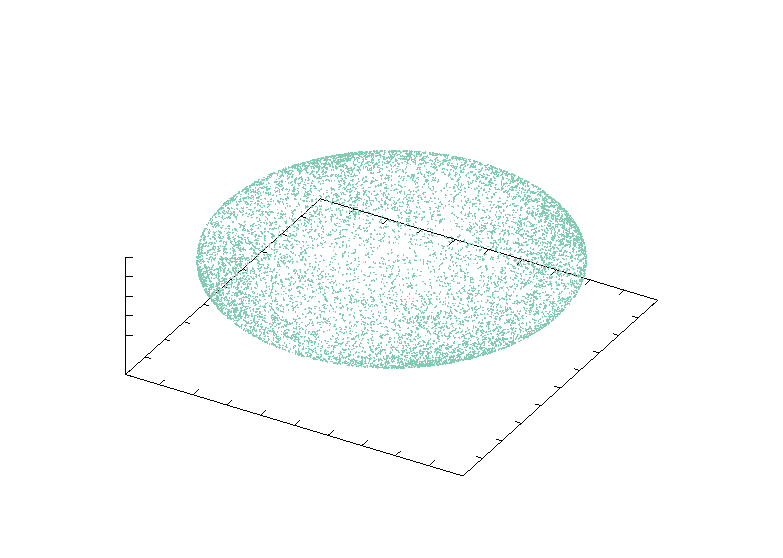
\includegraphics{nao_uniforme}}%
    \gplfronttext
  \end{picture}%
\endgroup
